

\tikzset{every picture/.style={line width=0.75pt}} %set default line width to 0.75pt        

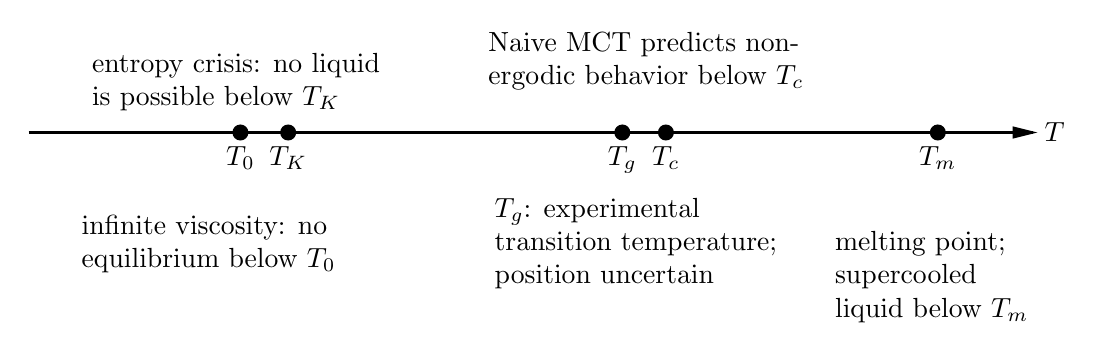
\begin{tikzpicture}[x=0.75pt,y=0.75pt,yscale=-1,xscale=1]
%uncomment if require: \path (0,378); %set diagram left start at 0, and has height of 378

%Straight Lines [id:da2866989210872881] 
\draw    (92,242) -- (576,242) ;
\draw [shift={(578,242)}, rotate = 180] [fill={rgb, 255:red, 0; green, 0; blue, 0 }  ][line width=0.08]  [draw opacity=0] (12,-3) -- (0,0) -- (12,3) -- cycle    ;
%Straight Lines [id:da4373164359721642] 
\draw    (194,242) ;
\draw [shift={(194,242)}, rotate = 0] [color={rgb, 255:red, 0; green, 0; blue, 0 }  ][fill={rgb, 255:red, 0; green, 0; blue, 0 }  ][line width=0.75]      (0, 0) circle [x radius= 3.35, y radius= 3.35]   ;
%Straight Lines [id:da9393368773961788] 
\draw    (217,242) ;
\draw [shift={(217,242)}, rotate = 0] [color={rgb, 255:red, 0; green, 0; blue, 0 }  ][fill={rgb, 255:red, 0; green, 0; blue, 0 }  ][line width=0.75]      (0, 0) circle [x radius= 3.35, y radius= 3.35]   ;
%Straight Lines [id:da5363038804777169] 
\draw    (530,242) ;
\draw [shift={(530,242)}, rotate = 0] [color={rgb, 255:red, 0; green, 0; blue, 0 }  ][fill={rgb, 255:red, 0; green, 0; blue, 0 }  ][line width=0.75]      (0, 0) circle [x radius= 3.35, y radius= 3.35]   ;
%Straight Lines [id:da22573584972311234] 
\draw    (378,242) ;
\draw [shift={(378,242)}, rotate = 0] [color={rgb, 255:red, 0; green, 0; blue, 0 }  ][fill={rgb, 255:red, 0; green, 0; blue, 0 }  ][line width=0.75]      (0, 0) circle [x radius= 3.35, y radius= 3.35]   ;
%Straight Lines [id:da8217101511374114] 
\draw    (399,242) ;
\draw [shift={(399,242)}, rotate = 0] [color={rgb, 255:red, 0; green, 0; blue, 0 }  ][fill={rgb, 255:red, 0; green, 0; blue, 0 }  ][line width=0.75]      (0, 0) circle [x radius= 3.35, y radius= 3.35]   ;

% Text Node
\draw (580,242) node [anchor=west] [inner sep=0.75pt]    {$T$};
% Text Node
\draw (194,247.4) node [anchor=north] [inner sep=0.75pt]    {$T_{\text{0}}$};
% Text Node
\draw (121,233) node [anchor=south west] [inner sep=0.75pt]   [align=left] {entropy crisis: no liquid \\is possible below $\displaystyle T_{\text{K}}$};
% Text Node
\draw (530,247.4) node [anchor=north] [inner sep=0.75pt]    {$T_{\text{m}}$};
% Text Node
\draw (479,335) node [anchor=south west] [inner sep=0.75pt]   [align=left] {melting point; \\supercooled \\liquid below $\displaystyle T_{\text{m}}$};
% Text Node
\draw (217,247.4) node [anchor=north] [inner sep=0.75pt]    {$T_{\text{K}}$};
% Text Node
\draw (116,311) node [anchor=south west] [inner sep=0.75pt]   [align=left] {infinite viscosity: no \\equilibrium below $\displaystyle T_{0}$};
% Text Node
\draw (378,247.4) node [anchor=north] [inner sep=0.75pt]    {$T_{\text{g}}$};
% Text Node
\draw (399,247.4) node [anchor=north] [inner sep=0.75pt]    {$T_{\text{c}}$};
% Text Node
\draw (312,192) node [anchor=north west][inner sep=0.75pt]   [align=left] {Naive MCT predicts non- \\ergodic behavior below $\displaystyle T_{\text{c}}$};
% Text Node
\draw (315,272) node [anchor=north west][inner sep=0.75pt]   [align=left] {$\displaystyle T_{\text{g}}$: experimental\\transition temperature;\\position uncertain};


\end{tikzpicture}
